\documentclass{article}
\usepackage{amsmath}
\usepackage{tikz}
\usetikzlibrary{arrows.meta}

\begin{document}

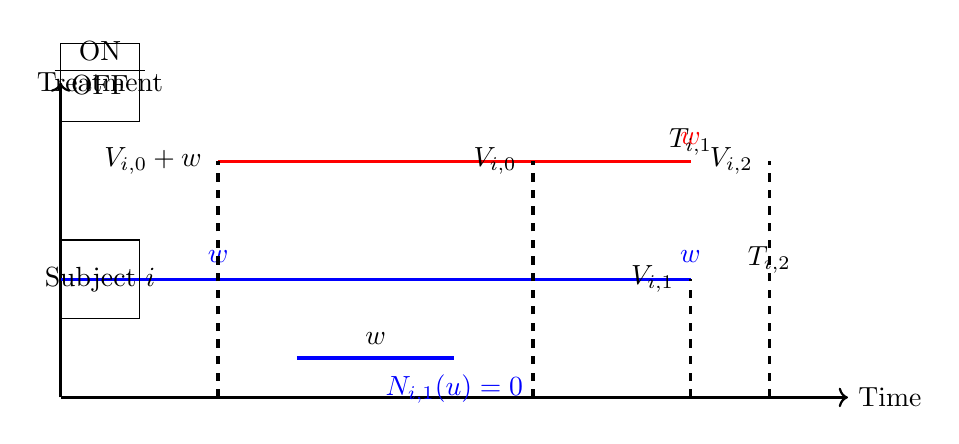
\begin{tikzpicture}
    % Draw the x-axis
    \draw[thick, ->] (0,0) -- (10,0) node[right] {Time};
    
    % Draw the y-axis
    \draw[thick, ->] (0,0) -- (0,4);
    
    % Draw the horizontal lines for each treatment state
    \draw[red, very thick] (2,3) -- (8,3) node[above=2pt] {$w$};
    \draw[blue, very thick] (0,1.5) -- (2,1.5) node[above=2pt] {$w$} -- (8,1.5) node[above=2pt] {$w$};

    % Draw the vertical lines for the start times of the treatment states
    \draw[dashed, very thick] (2,0) -- (2,3) node[left=2pt] {$V_{i,0} + w$};
    \draw[dashed, very thick] (6,0) -- (6,3) node[left=2pt] {$V_{i,0}$};
    \draw[dashed, very thick] (8,0) -- (8,1.5) node[left=2pt] {$V_{i,1}$};
    \draw[dashed, very thick] (9,0) -- (9,3) node[left=2pt] {$V_{i,2}$};

    % Draw the label for the treatment states
    \draw (0,3.5) rectangle (1,4.5);
    \node at (0.5,4) {Treatment};
    \node at (0.5,4.15) {\begin{tabular}{c} ON \\ \hline OFF \end{tabular}};
    
    % Draw the label for the subject
    \draw (0,1) rectangle (1,2);
    \node at (0.5,1.5) {Subject $i$};
    
    % Draw the label for the gap time T_{i,k}
    \node at (8,3.25) {$T_{i,1}$};
    \node at (9,1.75) {$T_{i,2}$};
    
    % Draw the label for the counting process N_{i,k}(u)
    \draw[blue, line width=1.5pt] (3,0.5) -- (5,0.5) node[below=2pt] {$N_{i,1}(u)=0$};
    \node at (4,0.75) {$w$};
\end{tikzpicture}

\end{document}